%%%%%%%%%%%%%%%%%%%%%%%%%%%%%%%%%%%%%%%%%%%%%%%%%%%%%%%%%%%%%%%%%%%%%%%%%%%%%%%%
% Chapter 1: Introducción
%%%%%%%%%%%%%%%%%%%%%%%%%%%%%%%%%%%%%%%%%%%%%%%%%%%%%%%%%%%%%%%%%%%%%%%%%%%%%%%%

%+++++++++++++++++++++++++++++++++++++++++++++++++++++++++++++++++++++++++++++++
% \section{Estado del arte}
% \label{1:sec:2}

% https://www.google.com/selfdrivingcar/
% https://en.wikipedia.org/wiki/Google_self-driving_car

En la actualidad la visión artificial está muy presente en sistemas de guiado
para vehículos autónomos, es decir, vehículos que son capaces de conducir sin
intervención humana. El objetivo de la visión artificial en este campo es
ofrecer una alternativa más segura y fiable frente al factor humano.

\begin{wrapfigure}{l}{0.5\textwidth}
  \vspace{-20pt}
  \begin{center}
    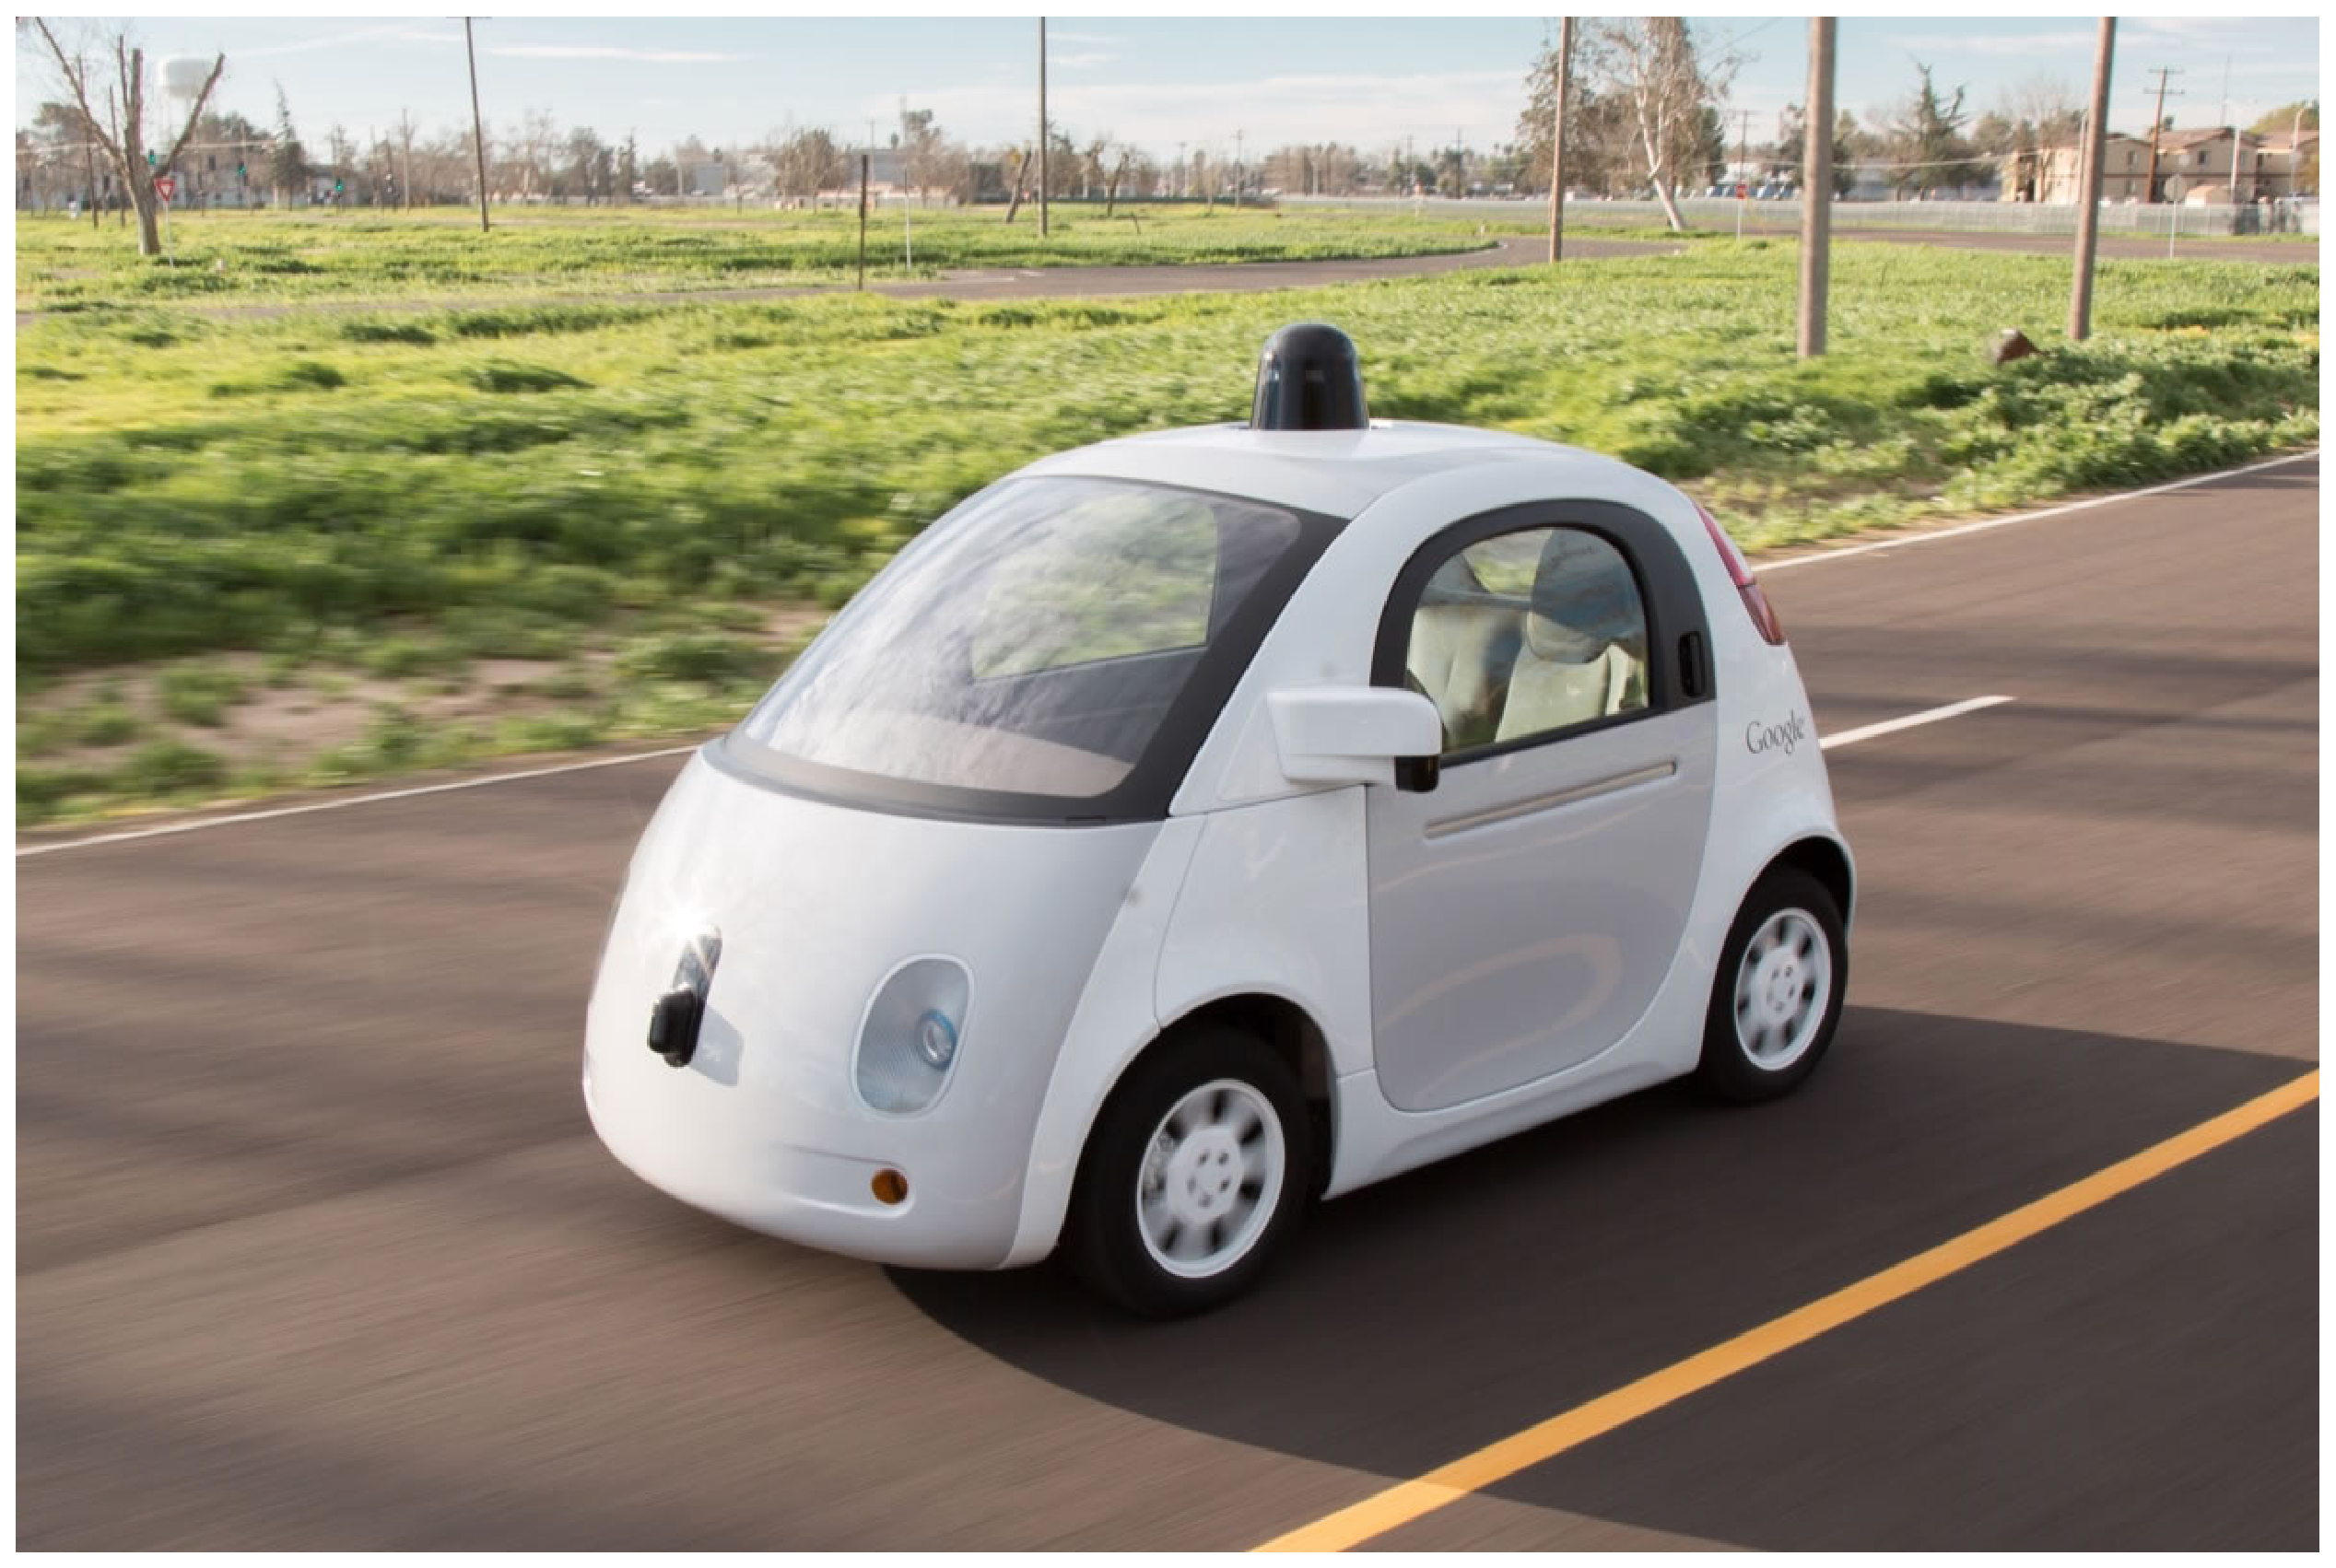
\includegraphics[width=0.48\textwidth]{images/cap1/GoogleSelf-DrivingCar.eps}
  \end{center}
  \vspace{-20pt}
  \caption{Google Self-Driving Car}
  \vspace{-10pt}
  \label{fig:GoogleSelf-DrivingCar}
\end{wrapfigure}

El ejemplo más conocido es el Google Self-Driving Car \cite{GoogleCar}, un
vehículo totalmente autónomo que tras varios años de investigación, desde 2011
ya es legal su circulación en varios estados de Estados Unidos.

Por otra parte, la Universidad de La Laguna cuenta con el proyecto VERDINO
\cite{ProjectPerenquen}, desarrollado por el Grupo de Robótica (GRULL). Se trata
de un vehículo similar al de Google que hace uso de sistemas láser, sistemas de
visión (tanto en el espectro visible como infrarrojo) y sistemas de odometría
óptica, entre otras características. Todo ello para ser capaz de detectar el
entorno que le rodea, y poder realizar una toma de decisiones mediante el uso de
diferentes algoritmos para llegar hasta un destino, al mismo tiempo que preocupa
por evitar los obstáculos que aparecen en su camino.

\begin{wrapfigure}{r}{0.5\textwidth}
  \vspace{-20pt}
  \begin{center}
    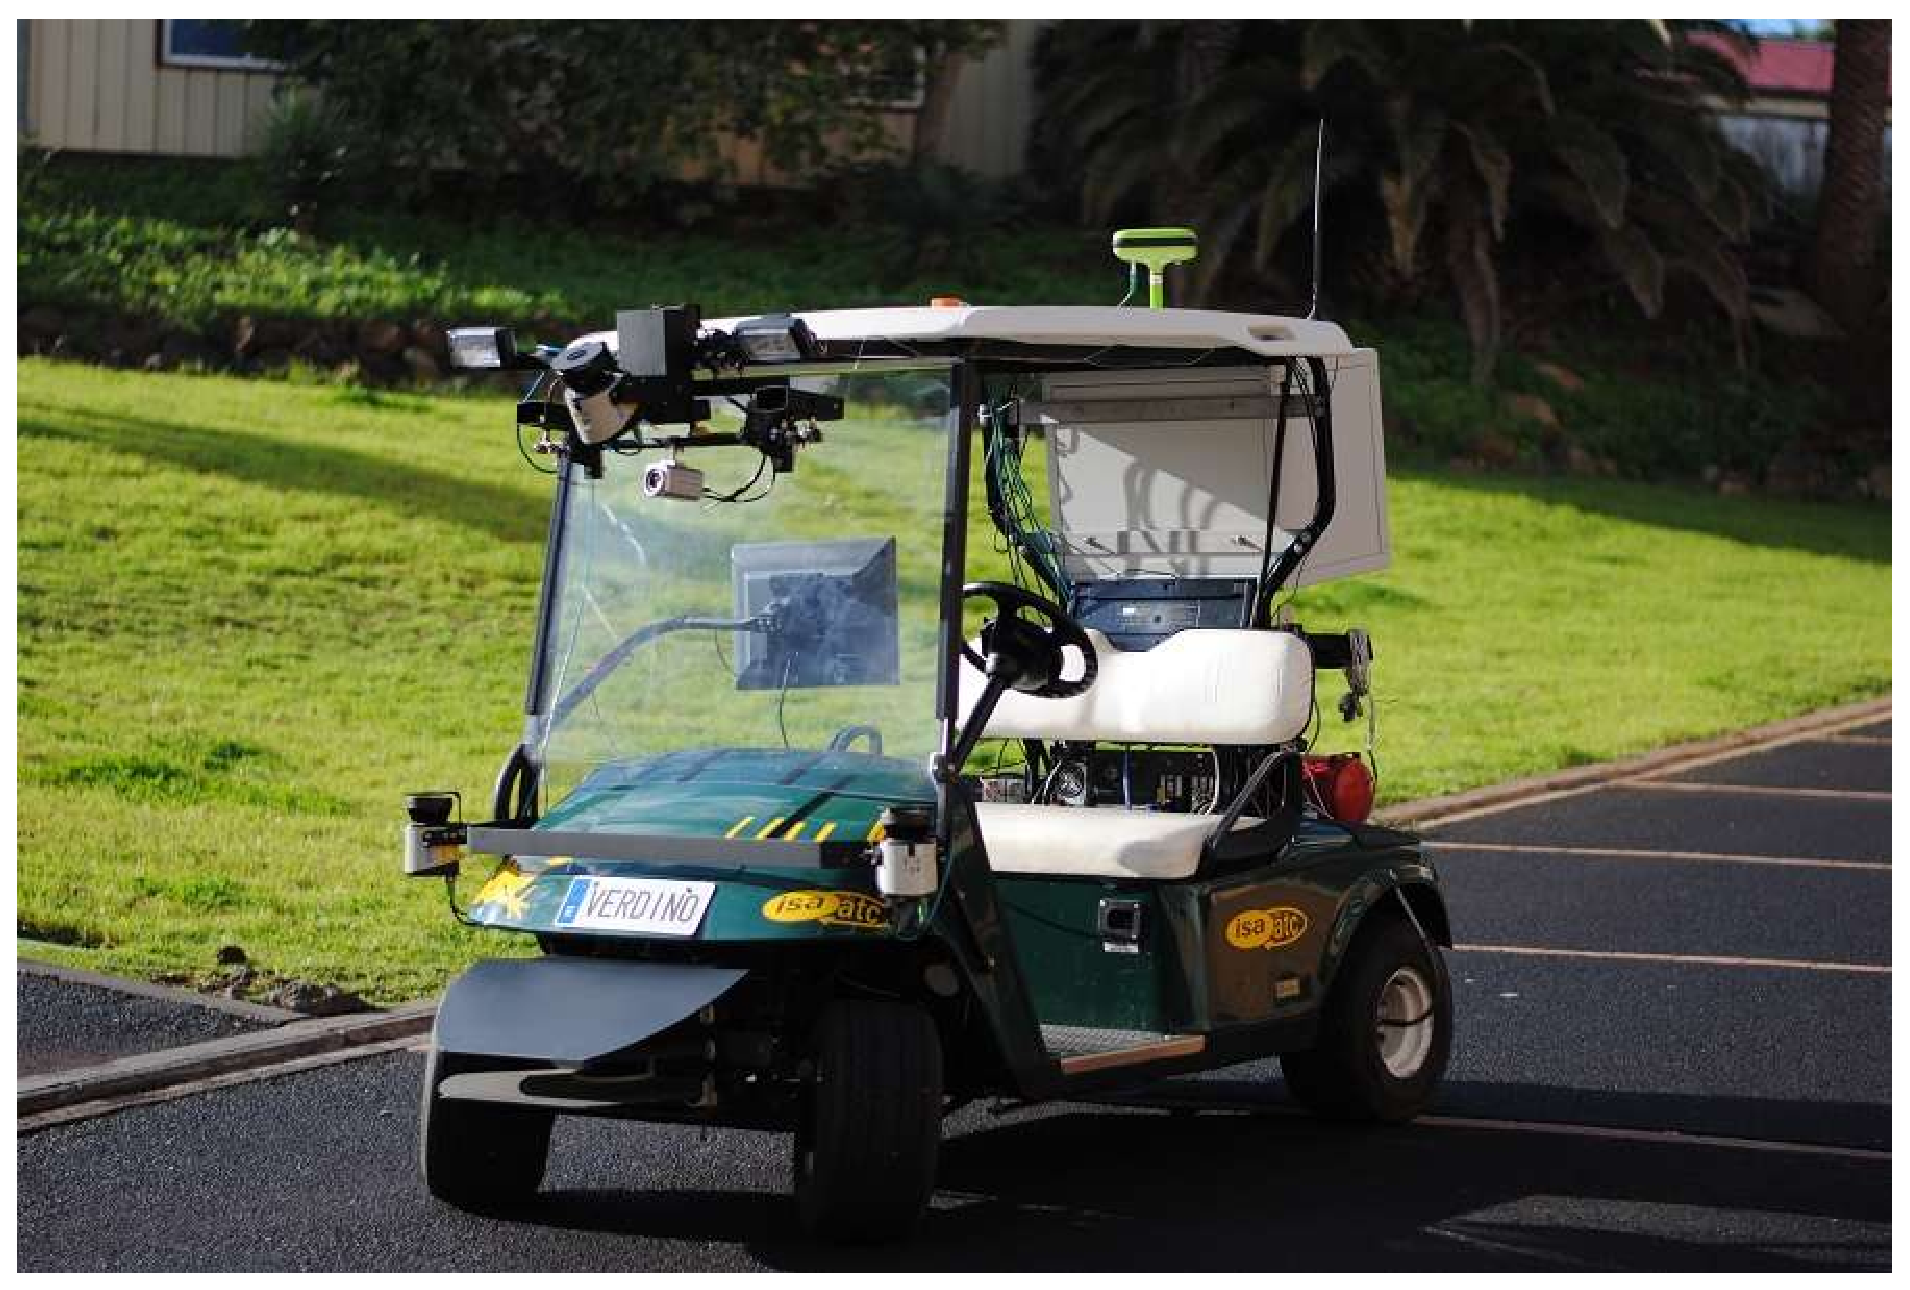
\includegraphics[width=0.48\textwidth]{images/cap1/Verdino.eps}
  \end{center}
  \vspace{-20pt}
  \caption{Proyecto VERDINO}
  \vspace{-10pt}
  \label{fig:ProyectoVERDINO}
\end{wrapfigure}

De momento es difícil predecir cuando se producirá la entrada masiva en el
mercado de este tipo de vehículos. Los dos proyectos mencionados anteriormente,
aunque fiables a pesar de seguir en desarrollo, hacen uso de tecnología poco
accesible para el público general debido a su elevado presupuesto.

Este problema abre las puertas a nuevas alternativas de investigación, a través
de tecnologías más económicas que todavía no se han explotado en este campo,
pero que son igual de válidas. Es el caso de los sistemas de visión
estereoscópica, que con solamente dos cámaras se puede obtener rica información
del entorno.

%+++++++++++++++++++++++++++++++++++++++++++++++++++++++++++++++++++++++++++++++
